\section{Problem}

Based on a grid world found in \cite{g:gridworld}, we have a $10\times 10$ grid, in which there are five obstacles (O), where an agent needs to find the exit (F). 


Let us have a Roomba in a five by five grid, and it notices that the battery is empty. The Roomba begins their journey towards their charging station (F). It so happens that the Roomba always registers that the battery needs to be charged on one of four possible starting positions (P). We want the Roomba to go back to their charging station as quickly as possible. However, there are a number of small items (O) that are on the floor. These are small enough that the Roomba can drive over the item, but the item will break. Another thing to note is the floor has been waxed recently, so the Roomba has a small chance of slipping. When slipping, the Roomba will move two tiles instead of one. The Roomba is only allowed to move north, east, south or west. See \figureref{f:10by10grid} for an overview of this problem

\begin{figure}[H]
\centering
\begin{tikzpicture}[cell/.style={rectangle,draw}]
  \matrix[
  matrix of nodes,
  execute at begin cell=\strut,
  execute at empty cell={\node{\strut};},
  nodes={cell,anchor=center,minimum width=0.75cm,minimum height=0.75cm}]{
& & & & & & & & & F\\
& & & & & &O & P & O & \\
& & & & & & & & & O \\
& & & & & & & & &  \\
& & & & & & & & &  \\
& & & & & & & & &  \\
& & & & & & & & &  \\
& P & & & & & & & &  \\
& P & P & & & & & & & O \\
& O & & & & & & & & \\};
\end{tikzpicture}
\caption{Overview for Roomba problem}
\label{f:10by10grid}
\end{figure}

The Roomba has the capability to observe 4 different things:
\begin{enumerate}
\item \texttt{start}: the Roomba needs to start the journey to the charging station.
\item \texttt{obstacle}: the Roomba has driven over an item.
\item \texttt{goal}: the Roomba has reached the charging station.
\item \texttt{notbad}: nothing of interest has happened. 
\end{enumerate} 

There are some different things we can let the Roomba learn in this situation. Let us start off simple. The Roomba has to reach the finish without driving over any small item. Thus, let our history-based reward function be:
\[\text{Reaching the goal, without encountering any obstacles} : 1\]
This can be represented in the following regular expression:
\[ \texttt{start notbad* goal} : 1\]
allowing us with the following reward controller:

\begin{figure}[H]
	\centering
		\begin{tikzpicture}[node distance=4cm,on grid,auto]
			\node[initial,state] (1) 			{$q_0/0$};
			\node[state] (2) [right=of 1]		{$q_1/0$};
			\node[state] (3) [right=of 2]		{$q_2/1$};
			\node[state] (4) [below=of 2]		{$q_3/0$};
			\path[->] 	(1) edge[] 	node [above] {\texttt{start}}			(2)
							edge[bend right]  node [left,text width=1cm,align=center] {\texttt{notbad, obstacle, goal}}			(4)
						(2) edge[loop above] 	node [above,text width=1cm,align=center] {\texttt{notbad}}			()
							edge[] 	node [above] {\texttt{goal}}			(3)
							edge[] node [left,text width=1cm,align=center] {\texttt{obstacle, goal}} (4)
						(3) edge[bend left] 	node [right,text width=1cm,align=center] {\texttt{start, notbad, goal, goal}}	(4);
	\end{tikzpicture}
\caption{Reward Controller for reinforced learning}
	\label{f:rc_gridworld}
\end{figure}

Logically speaking, there will not occur a transition after the \texttt{goal} has been observed by designation of the model. However, since the reward controller is a deterministic automaton, we specify this. 

To solve this, we find a policy for maximizing the involved rewards to ensure the Roomba finds a policy to reach the goal without hitting any obstacles. \\


Another way to tackle the problem of reaching the charging station without hitting any obstacle, is to give a penalty for observing an obstacles. A simple way to approximate this problem would be to simply specify in the \texttt{prism}-program that every time you observe an obstacle, you get a penalty of 50 for example. To find a policy for this, we ask to minimalize the involved costs.\\

However, such a problem is not always linear in real life. A more realistic approach for giving penalties would be to give a small penalty for the first occurence, but higher penalties for when it happens more than once.

For example, if the Roomba drives over an object you might still be able to fix the object. But, if the Roomba drives over multiple ones, it will be easier to just throw all of the items out, resulting in a much higher cost. To approximate this, let's take a look at the following approach. So instead of minimizing the involved costs, we want the maximize the profit we get for not having to fix or throw away the items involved.

\begin{figure}[H]
	\centering
		\begin{tikzpicture}[node distance=3.5cm,on grid,auto]
			\node[initial,state] (1) 			{$q_0/0$};
			\node[state] (2) [right=of 1]		{$q_1/0$};
			\node[state] (3) [right=of 2]		{$q_2/0$};
			\node[state] (4) [right=of 3]		{$q_3/0$};
			\node[state] (5) [right=of 4]		{$q_4/0$};
			\node[state] (6) [below=of 2]        {$q_5/100$};
			\node[state] (7) [below=of 3]        {$q_5/50$};
			\node[state] (8) [below=of 4]        {$q_6/10$};
			\node[state] (9) [below=of 5]        {$q_6/0$};
			\path[->] 	(1) edge[] 	node [above] {\texttt{start}}			(2)
						(2) edge[loop above] 	node [above,text width=1cm,align=center] {\texttt{notbad}}			()
							edge[] 	node [above] {\texttt{obstacle}}			(3)
							edge[] 	node [left] {\texttt{goal}}			(6)
						(3) edge[loop above] 	node [above,text width=1cm,align=center] {\texttt{notbad}}			()
							edge[] 	node [above] {\texttt{obstacle}}			(4)
							edge[] 	node [left] {\texttt{goal}}			(7)
						(4) edge[loop above] 	node [above,text width=1cm,align=center] {\texttt{notbad}}			()
							edge[] 	node [above] {\texttt{obstacle}}			(5)
							edge[] 	node [left] {\texttt{goal}}			(8)
						(5) edge[loop above] 	node [above,text width=1cm,align=center] {\texttt{notbad}}			()
							edge[] 	node [left] {\texttt{goal}}			(9);
	\end{tikzpicture}
\caption{Reward Controller for broken obstacles}
	\label{f:rc_2}
\end{figure}

In \figureref{f:rc_2} some transitions are missing. Whenever a transition occurs that isn't specified it will go to a dump state, one that has a zero reward encoded.




\section{Results}
For testing this scenario, we have to pick the maximum observation sequence length $T$ as we have seen in \defref{d:limited_pomdp}. 
We have run the benchmark toolchain for creating policies for POMDPs\cite{g:toolchain} on a system which runs on \texttt{Ubuntu 20.04.3 LTS}. The system has a \texttt{Intel Core i3-6006U} processor and 4GB of RAM.

This tool solves the POMDP given a specific property that we want to check. For our problem we want to find the maximum expected reward after reading a sequence up to length $T$, given the reward function as stated above. The tool finds this value and then finds a policy that complies with this value. A pMC will be generated for finding an optimal policy. The size of this is represented in number of states and number of transitions. 

The empty slots depict the fact that the size of the pMC was too big to be solved. \todo{move tables to appendix?}
%\begin{sidewaystable}
\centering
\begin{tabular}{|r|c|c|c|c|c|c|c|c|c|c|}
\hline
T & 50 & 100 & 150 & 200 & 250 & 300 & 350 & 400 & 450 & 500 \\ \hline
Solver time (s) & 2.28 & 6.68 & 11.96 & 18.77 & 26.62 & 35.84 & 46.69 & 58.40 & 71.42 & - \\
Encoding time (s) & 148.55 & 364.16 & 525.13 & 695.75 & 880.37 & 1055.46 & 1242.38 & 1422.13 & 1603.73 & - \\
\# pMC states & 32432 & 73532 & 114632 & 155732 & 196832 & 237932 & 279032 & 320132 & 361232 & 402332 \\
\# pMC transitions & 63222 & 143442 & 223662 & 303882 & 384102 & 464322 & 544542 & 624762 & 704982 & 785202 \\
Result & 0.22608 & 0.22625 & 0.22625 & 0.22625 & 0.22625 & 0.22625 & 0.22625 & 0.22625 & 0.22625 & 0.22625 \\	 \hline
\end{tabular}
\caption{Results for $N=5$}


\vspace{2\baselineskip}
\begin{tabular}{|r|c|c|c|c|c|c|c|c|c|c|}
\hline
T & 5 & 10 & 15 & 20 & 25 & 30 & 35 & 40 & 45 & 50\\ \hline
Solver time (s) & 0.16 & 2.95 & 8.21 & 15.11 & 24.17 & 35.22 & 49.19 & 61.07 & 77.37 & - \\
Encoding time (s) & 
11.95 & 172.79 & 383.88 & 595.19 & 805.52 & 1025.71 & 1232.19 & 1425.90 & 1638.00 & - \\
\# pMC states & 2740 & 39908 & 88268 & 136628 & 184988 & 233348 & 281708 & 330068 & 378428 & 426788 \\
\# pMC transitions & 5223 & 77819 & 172564 & 267309 & 362054 & 456799 & 551544 & 646289 & 741034 & 835779 \\
Result & 
0.034790 & 0.20539 & 0.21518 & 0.21620 & 0.21636 & 0.21639 & 0.21640 & 0.21640 & 0.21640 & 0.21640 \\ \hline
\end{tabular}
\caption{Results for $N=10$}

\end{sidewaystable}


%\begin{figure}[H]
\centering
\begin{subfigure}[H]{0.4\textwidth}
	\centering

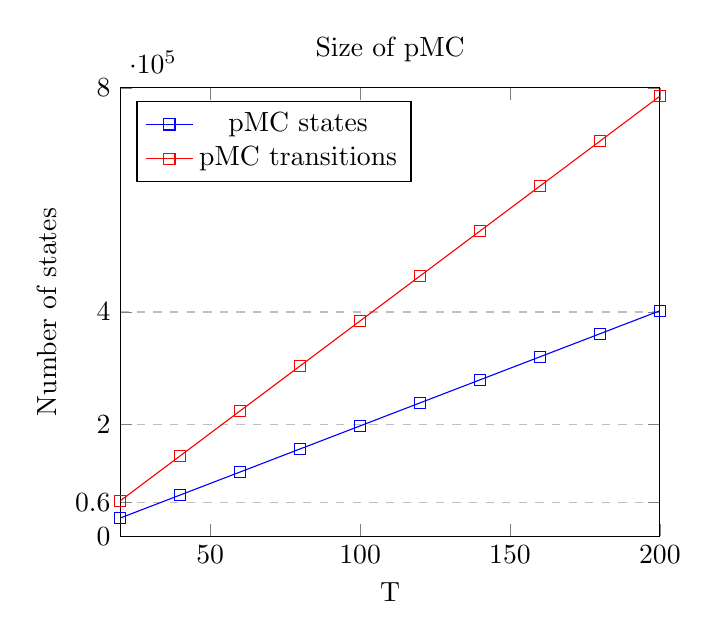
\begin{tikzpicture}
\begin{axis}[
    title={Size of pMC},
    xlabel={T},
    ylabel={Number of states},
    xmin=20, xmax=200,
    ymin=0, ymax=800000,
    xtick={0,50,100,150,200},
    ytick={0,200000,400000,60000,800000},
    legend pos=north west,
    ymajorgrids=true,
    grid style=dashed,
]

\addplot[
    color=blue,
    mark=square,
    ]
    coordinates {
    (20,32432)(40,73532)(60,114632)(80,155732)(100,196832)(120,237932)(140,279032)(160,320132)(180,361232)(200,402332)
    };
    
\addplot[
    color=red,
    mark=square,
    ]
    coordinates {
    (20,63222)(40,143442)(60,223662)(80,303882)(100,384102)(120,464322)(140,544542)(160,624762)(180,704982)(200,785202)
    };
    \legend{pMC states, pMC transitions}

\end{axis}
\end{tikzpicture}
\end{subfigure}
\hfill
\begin{subfigure}[H]{0.4\textwidth}
	\centering
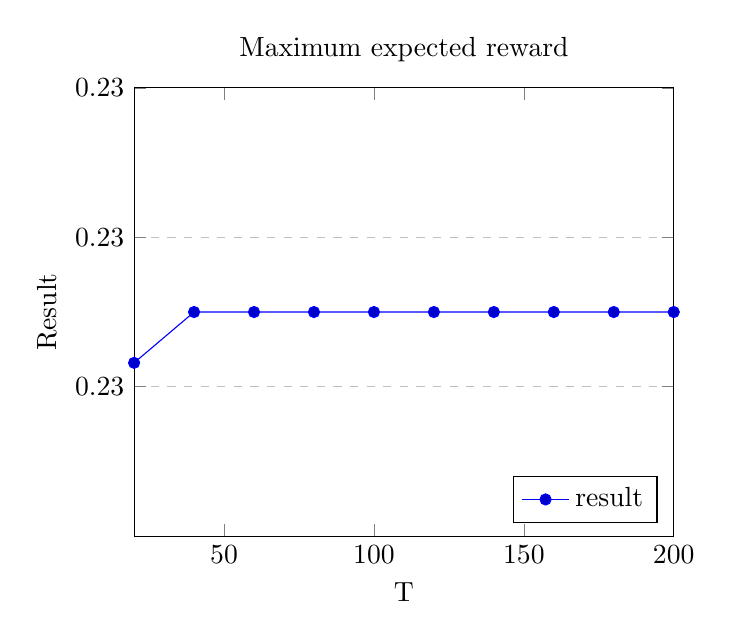
\begin{tikzpicture}

\begin{axis}[
    title={Maximum expected reward},
    xlabel={T},
    ylabel={Result},
    xmin=20, xmax=200,
    ymin=0.2255,ymax=0.227,
    xtick={0,50,100,150,200},
    ytick={0.226,0.2265,0.227},
    legend pos=south east,
    ymajorgrids=true,
    grid style=dashed]    
\addplot
    coordinates {
    (20,0.22608)(40,0.22625)(60,0.22625)(80,0.22625)(100,0.22625)(120,0.22625)(140,0.22625)(160,0.22625)(180,0.22625)(200,0.22625)
    };
    \legend{result}
    
\end{axis}
\end{tikzpicture}
\end{subfigure}

\begin{subfigure}[H]{0.4\textwidth}
	\centering
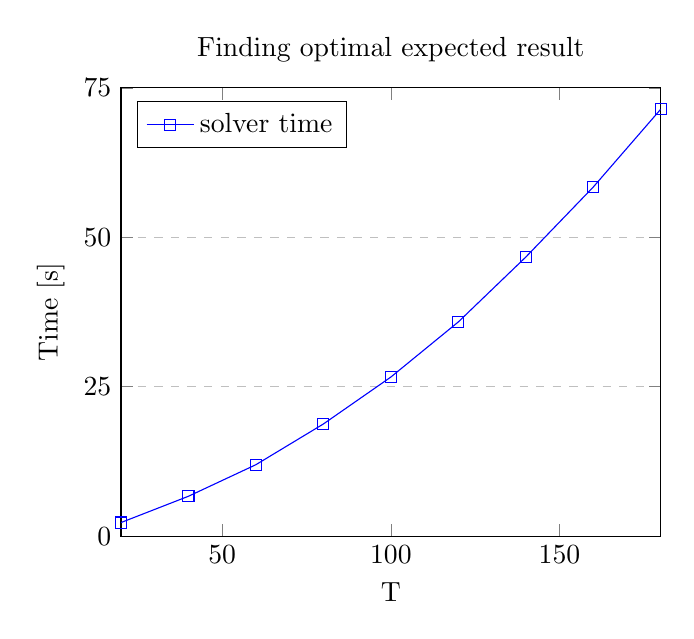
\begin{tikzpicture}
\begin{axis}[
    title={Finding optimal expected result},
    xlabel={T},
    ylabel={Time [s]},
    xmin=20, xmax=180,
    ymin=0, ymax=75,
    xtick={0,50,100,150,200},
    ytick={0,25,50,75},
    legend pos=north west,
    ymajorgrids=true,
    grid style=dashed,
]

\addplot[
    color=blue,
    mark=square,
    ]
    coordinates {
    (20,2.28)(40,6.68)(60,11.96)(80,18.77)(100,26.62)(120,35.84)(140,46.69)(160,58.40)(180,71.42)
    };
    \legend{solver time}

\end{axis}
\end{tikzpicture}
\end{subfigure}
\hfill
\begin{subfigure}[H]{0.4\textwidth}
	\centering
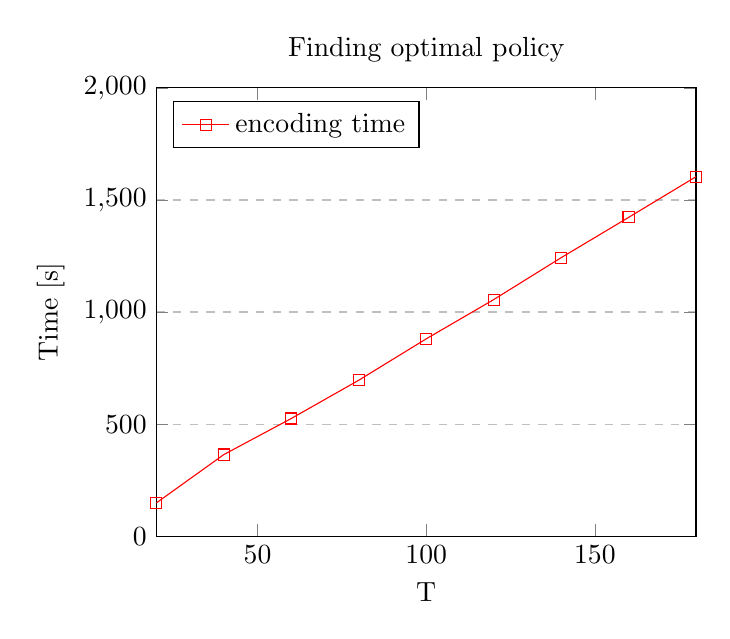
\begin{tikzpicture}
\begin{axis}[
    title={Finding optimal policy},
    xlabel={T},
    ylabel={Time [s]},
    xmin=20, xmax=180,
    ymin=0, ymax=2000,
    xtick={0,50,100,150},
    ytick={0,500,1000,1500,2000},
    legend pos=north west,
    ymajorgrids=true,
    grid style=dashed,
]
    
\addplot[
    color=red,
    mark=square,
    ]
    coordinates {
    (20,148.55)(40,364.16)(60,525.13)(80,695.75)(100,880.37)(120,1055.46)(140,1242.38)(160,1422.13)(180,1603.73)
    };
    \legend{encoding time}
    
\end{axis}
\end{tikzpicture}
\end{subfigure}
\caption{Results for $N=5$}
\end{figure}









\begin{figure}[H]
\centering
\begin{subfigure}[H]{0.4\textwidth}
	\centering

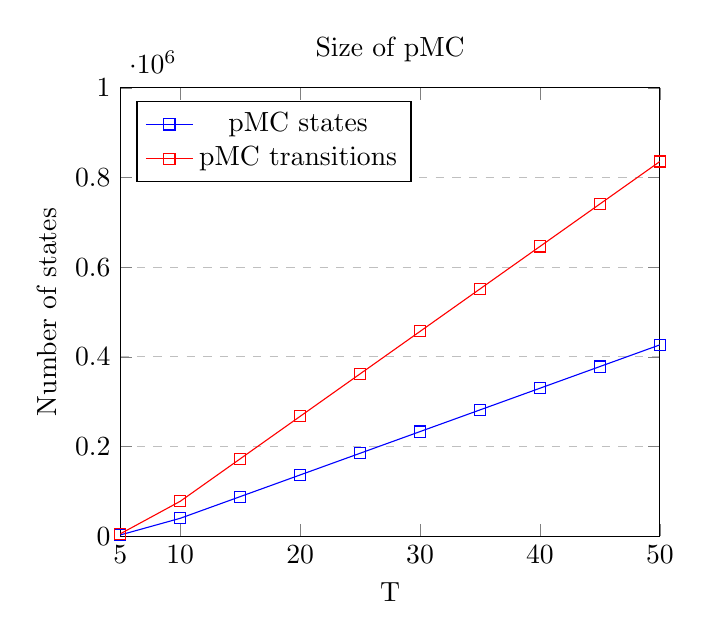
\begin{tikzpicture}
\begin{axis}[
    title={Size of pMC},
    xlabel={T},
    ylabel={Number of states},
    xmin=5, xmax=50,
    ymin=0, ymax=1000000,
    xtick={5,10,20,30,40,50},
    ytick={0,200000,400000,600000,800000,1000000},
    legend pos=north west,
    ymajorgrids=true,
    grid style=dashed,
]

\addplot[
    color=blue,
    mark=square,
    ]
    coordinates {
(5,2740)(10,39908)(15,88268)(20,136628)(25,184988)(30,233348)(35,281708)(40,330068)(45,378428)(50,426788)
    };
    
\addplot[
    color=red,
    mark=square,
    ]
    coordinates {
(5,5223)(10,77819)(15,172564)(20,267309)(25,362054)(30,456799)(35,551544)(40,646289)(45,741034)(50,835779)
    };
    \legend{pMC states, pMC transitions}
    
\end{axis}
\end{tikzpicture}
\end{subfigure}
\hfill
\begin{subfigure}[H]{0.4\textwidth}
	\centering
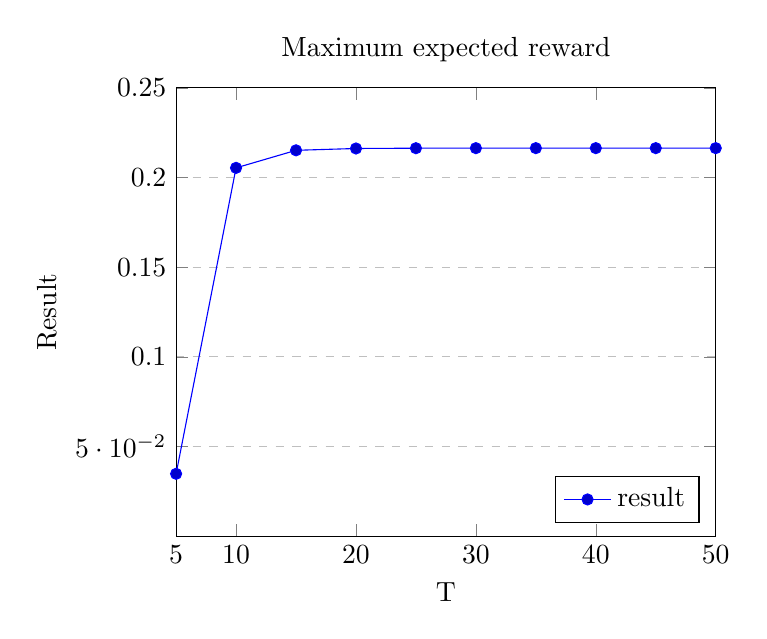
\begin{tikzpicture}

\begin{axis}[
    title={Maximum expected reward},
    xlabel={T},
    ylabel={Result},
    xmin=5, xmax=50,
    ymin=0, ymax=0.25,
    xtick={5,10,20,30,40,50},
    ytick={0.05,0.1,0.15,0.2,0.25},
    legend pos=south east,
    ymajorgrids=true,
    grid style=dashed,
]
    
\addplot
    coordinates {
(5,0.034790)(10,0.20539)(15,0.21518)(20,0.21620)(25,0.21636)(30,0.21639)(35,0.21640)(40,0.21640)(45,0.21640)(50,0.21640)
    };
    \legend{result}
    
\end{axis}
\end{tikzpicture}
\end{subfigure}

\begin{subfigure}[H]{0.4\textwidth}
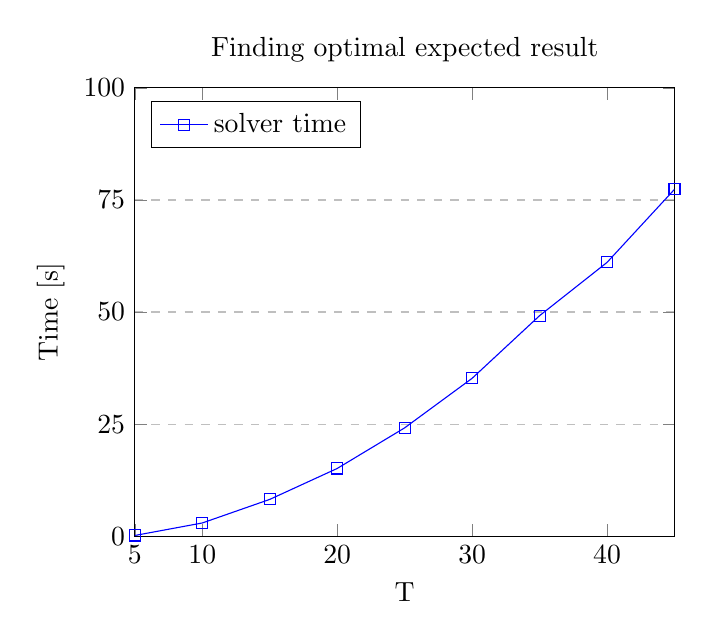
\begin{tikzpicture}
\begin{axis}[
	title={Finding optimal expected result},
    xlabel={T},
    ylabel={Time [s]},
    xmin=5, xmax=45,
    ymin=0, ymax=100,
    xtick={5,10,20,30,40,50},
    ytick={0,25,50,75,100},
    legend pos=north west,
    ymajorgrids=true,
    grid style=dashed,
]

\addplot[
    color=blue,
    mark=square,
    ]
    coordinates {
(5,0.16)(10,2.95)(15,8.21)(20,15.11)(25,24.17)(30,35.22)(35,49.19)(40,61.07)(45,77.37)
    };
    \legend{solver time}
    
\end{axis}
\end{tikzpicture}
\end{subfigure}
\hfill
\begin{subfigure}[H]{0.4\textwidth}
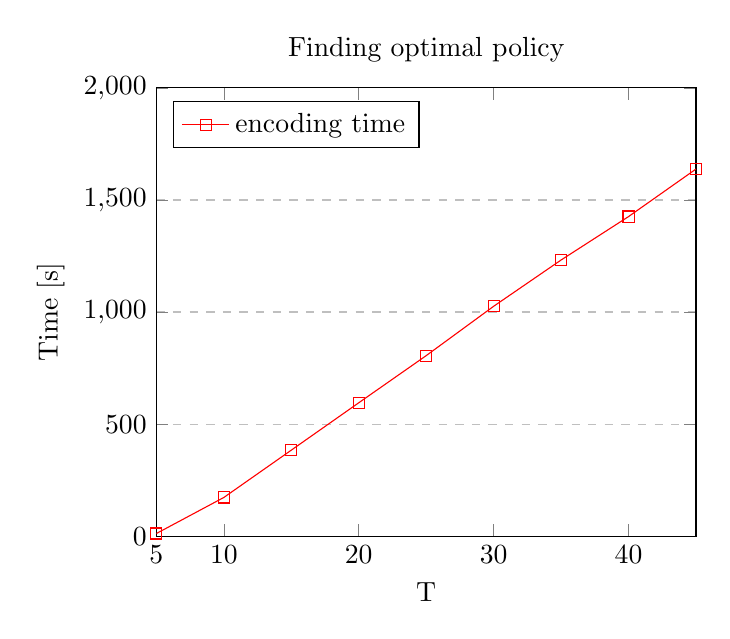
\begin{tikzpicture}
\begin{axis}[
title={Finding optimal policy},
    xlabel={T},
    ylabel={Time [s]},
    xmin=5, xmax=45,
    ymin=0, ymax=2000,
    xtick={5,10,20,30,40,50},
    ytick={0,500,1000,1500,2000},
    legend pos=north west,
    ymajorgrids=true,
    grid style=dashed,
]
    
\addplot[
    color=red,
    mark=square,
    ]
    coordinates {
(5,11.95)(10,172.79)(15,383.88)(20,595.19)(25,805.52)(30,1025.71)(35,1232.19)(40,1425.90)(45,1638.00)
    };
    \legend{encoding time}
    
\end{axis}
\end{tikzpicture}
\end{subfigure}
\caption{Results for $N=10$}
\end{figure}
For $N=5$ we observe that the maximum expected reward had been reached already when $T=50$.

For $N=10$ we can see that the maximum expected reward has been reached for when $T=35$. This can be decreased if we allow for a certain error margin.

The sizing of the pMC that is needed to solve for the policy for optaining the maximum expected reward seems to be linear, in terms of states as wel ass transitions. Since the solver for finding the optimal expected reward is a bit more than linear, it would be pertinent to find the smallest $T$ possible, given a certain error margin for the expected maximum reward.
